% Drawing 136/17-1 -- folder 136, batch 17, archive page 326 (PDF page 327).
% Transcription: un disque hachuré marqué d'un point $\tilde x$, dans un carré, avec une boucle qui en sort
% Kind: hatched disc with point x~ in a square, with a loop. Method 2 (schematic redraw from the facsimile). Status: ok.
% Notes: A hatched disc with a heavy rim, the point x~ in it (and two small dots), inside a roughly drawn square; a loop leaves the disc to the right and goes out of the square.
% Coordinates: 1 unit = 1 mm = 1/100 of the crop width (bbox in page fractions: [0.24, 0.47, 0.36, 0.53]).
% Redrawn by Claude (claude-opus-5-5), issue #73, 2026-11-07; not checked by a human; not compiled (no TeX in the session).
% Rights: reproduces part of the work -- behind RENDER_TRANSCRIPTS, never published by itself.
\documentclass[tikz,border=3pt]{standalone}
\usepackage{amsmath,amssymb}
\usetikzlibrary{patterns,arrows.meta}
\tikzset{pencil/.style={black!45}, struck/.style={black!35}, mark/.style={circle,draw,inner sep=1.3pt}, pt/.style={circle,fill,inner sep=0.9pt}, opt/.style={circle,draw,fill=white,inner sep=1.1pt}}
\begin{document}
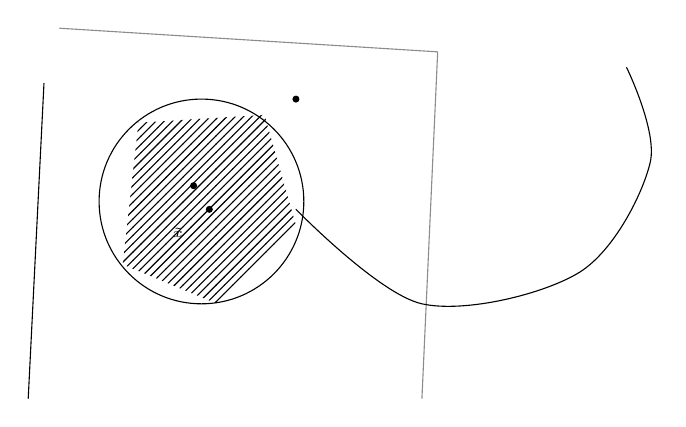
\begin{tikzpicture}[x=1mm,y=1mm,line cap=round,line join=round,font=\scriptsize]
\draw[pencil] (20,-5) -- (68,-8) -- (66,-52);
\draw (18,-12) -- (16,-52);
\draw (38,-27) circle[radius=13];
\fill[pattern=north east lines] (30,-17) -- (46,-16) -- (50,-30) -- (40,-40) -- (28,-35) -- cycle;
\node[pt] at (39,-28) {};
\node[pt] at (37,-25) {};
\node[pt] at (50,-14) {};
\node[inner sep=1pt] at (35,-31) {\tiny $\tilde x$};
\draw plot[smooth, tension=0.55] coordinates {(50,-28) (66,-40) (86,-36) (95,-22) (92,-10)};
\end{tikzpicture}
\end{document}
